% Scalar instruction entry source: tools/generate_scalar_instruction_catalog.py.
\subsection{\texttt{CMP.GEUI}}
\label{sec:scalar-cmp_geui}
\index{CMP.GEUI@\texttt{CMP.GEUI}}
\begin{sloppypar}\noindent\textbf{Purpose.} Performs an unsigned greater-than-or-equal comparison between SrcL and the immediate operand and writes 1 or 0 to RegDst.\end{sloppypar}\smallskip
\noindent\textbf{Syntax.}\par
\begin{lstlisting}[style=ptoscalarcode]
cmp.geui SrcL, uimm, ->RegDst
\end{lstlisting}
\noindent\textbf{Encoding.}\par
\noindent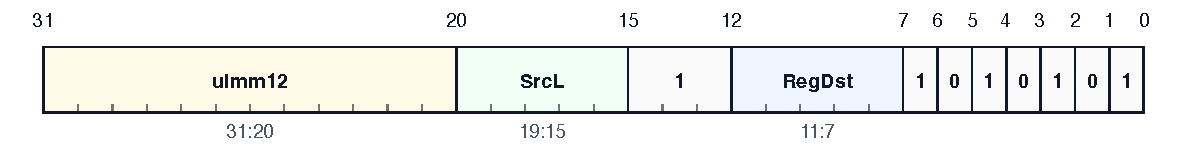
\includegraphics[width=\textwidth]{figs/encoding/scalar_instruction_entries/enc_cmp_geui.pdf}\par\smallskip
\begin{description}[leftmargin=0.18\linewidth,style=nextline]
\item[Format] \texttt{L32} \texttt{32-bit} scalar word.
\item[Pattern] \texttt{.................111.....1010101}.
\end{description}
\noindent\textbf{Classification.}\par
\begin{description}[leftmargin=0.18\linewidth,style=nextline]
\item[Category] Branch, Compare, and PC Control.
\item[Family] Compare Instruction.
\item[Execution class] \texttt{BRU}; uop\_kind=BRU, bru\_kind=CMP.
\end{description}
\noindent\textbf{Operand fields.}\par
\begin{description}[leftmargin=0.18\linewidth,style=nextline]
\item[\texttt{RegDst}] Bits \texttt{11:7 (5b)}. 5-bit scalar destination register that receives the boolean compare result, encoded as 1 for true and 0 for false; X0 discards the write.
\item[\texttt{SrcL}] Bits \texttt{19:15 (5b)}. 5-bit scalar source register used as the left operand of the comparison.
\item[\texttt{uimm12}] Bits \texttt{31:20 (12b)}. 12-bit unsigned immediate operand consumed directly by the operation.
\end{description}
\noindent\textbf{Operation.}\par
\begin{lstlisting}[style=ptoscalarcode]
imm = ZeroExtend(uimm)
result = (Read(SrcL) >= imm  // unsigned) ? 1 : 0
Write(RegDst, result)
\end{lstlisting}
\Needspace{0.08\textheight}
